\documentclass{article}
\usepackage{color}
\usepackage{soul}
\usepackage{multirow}
\usepackage{pgfplots}
\usepackage{ifthen}
\usepackage{tikz}
\usepackage[UTF8]{ctex}
\usepackage[left=2cm,right=2cm,top=2cm,bottom=2cm]{geometry}
\geometry{a4paper}
\usepackage{tikz}
\usetikzlibrary{chains}
\newcommand{\diff}{\mathop{}\!\mathrm{d}}
\usepackage{appendix} 
\usepackage{lipsum}
\usepackage{listings}
\usepackage{diagbox}
\usepackage{pdfpages}
\usepackage{xcolor}
\usepackage{pdflscape}
\usepackage{soul}
\usepackage{booktabs}
\usepackage{longtable}
\usepackage[most]{tcolorbox}
\newtcolorbox{mycolorbox}[1][]{
  sharp corners,
  colback=white, 
  colframe=black, 
  coltext=blue, 
  boxsep=5pt, 
  left=2pt, 
  right=2pt, 
  top=1pt, 
  bottom=1pt,
  breakable,
  #1 
}
\usepackage{subcaption}
\lstset{
    backgroundcolor=\color{gray!20},
    basicstyle=\ttfamily,
    commentstyle=\color{darkgray}\ttfamily,
    stringstyle=\color{red},
    showstringspaces=false,
    numbers=left,
    numberstyle=\tiny\color{gray},
    stepnumber=1,
    numbersep=10pt,
    tabsize=4,
    showspaces=false,
    showtabs=false,
    frame=single,
    captionpos=b,
    breaklines=true,
    breakatwhitespace=false,
    escapeinside={\%*}{*)},
    xleftmargin=\parindent,
    xrightmargin=\parindent,
}
\lstdefinestyle{dockerstyle}{
    language=bash,
    keywordstyle=\color{blue}\bfseries,
    morekeywords={FROM, RUN, CMD, LABEL, EXPOSE, ENV, ADD, COPY, ENTRYPOINT, VOLUME, USER, WORKDIR, ARG, ONBUILD},
}
\lstdefinestyle{pythonstyle}{
    language=Python,
    keywordstyle=\color{blue}\bfseries,
    morekeywords={import, from, as, def, return, class, self, if, elif, else, while, for, try, except, with},
}
\lstdefinestyle{cstyle}{
    language=C,
    keywordstyle=\color{blue}\bfseries,
    morekeywords={size_t, printf},
}
\lstdefinestyle{bashstyle}{
    language=bash,
    keywordstyle=\color{blue}\bfseries,
    morekeywords={if, then, else, fi, for, in, do, done, echo, exit, return, function},
    commentstyle=\color{green}\ttfamily,
}
\usepackage{algorithm}
\usepackage{algpseudocode}
\renewcommand{\algorithmicrequire}{\textbf{Input:}}  
\renewcommand{\algorithmicensure}{\textbf{Output:}}  
\usepackage{amsmath}
\usepackage{amsthm}
\DeclareMathOperator{\sigm}{sigm}
\usepackage{graphicx}
\usepackage{float}
\renewcommand{\vec}[1]{\boldsymbol{#1}}
\usepackage{amssymb}
\usepackage{booktabs} 
\usepackage{hyperref}
\usepackage{titlesec}
\usepackage{caption}
\usepackage{fontspec}
\usepackage{xeCJK}
\setCJKmainfont{SimSun} 
\title{\Huge CUDA\&CUDA和OpenMP混合编程实验报告}
\author{21121178 王士博}
\begin{document}
\maketitle
\section{实验环境}
\textbf{Windows11 Professional 22H2 x64:} \\
\\
\indent \indent \indent \begin{minipage}[H]{0.7\textwidth}
    \begin{itemize}
        \item \textbf{处理器:}Intel(R) Core(TM) i7-11800H CPU @ 4.60GHz 16线程
        \item \textbf{内存:}32.0 GB
        \item \textbf{显卡:}NVIDIA GeForce RTX 3070
        \item \textbf{显卡驱动版本:}11.6
        \item \textbf{编程语言:}C++
        \item \textbf{编译器:}nvcc
        \item \textbf{编程平台:}Visual Studio 2019
    \end{itemize}
\end{minipage}
\section{实验目的}
\begin{enumerate}
    \item 了解CUDA的安装方式和注意问题。通过简洁明了地列出CUDA安装的步骤和关键注意事项,目的在于为CUDA新用户提供一个清晰、易于遵循的安装指南。这不仅帮助用户高效完成CUDA环境的配置,也旨在通过分享实践经验,降低并行编程技术的入门门槛,尤其是对于那些首次尝试在个人计算机上进行CUDA编程的用户。
    \item 使用CUDA或者CUDA和OpenMP混合编程实现矩阵乘法并且根据自己的电脑配置进行优化。现矩阵乘法的CUDA版本以及可能的OpenMP-CUDA混合编程版本,并基于个人机器的具体配置,从多个角度对比其加速比。此实验目的在于探究CUDA和OpenMP-CUDA混合编程技术在执行复杂运算任务时的性能差异,以及评估在不同计算资源配置下的执行效率。通过实验,旨在深入理解GPU并行计算的优势与局限,以及混合编程模式在提升计算性能方面的潜力,同时,通过附上源码,增加实验的可重复性和透明度,为并行计算领域的学习者和研究者提供参考。
\end{enumerate}
\section{实验步骤}
\subsection{CUDA的安装}
\begin{enumerate}
    \item \textbf{下载CUDA Toolkit:}这一步需要区分任务性质,首先确定是进行深度学习还是
    进行CUDA编程,如果只是进行深度学习,那么没没有必要安装完整的CUDA Toolkit,只需使用conda
    在虚拟环境中安装cudatoolkit即可,步骤如(b);如果是进行CUDA编程,那么需要下载完整的CUDA Toolkit如步骤(a)。
    \[
\text{CUDAToolkit} =
\left\{
\begin{array}{ >{\displaystyle}l >{\displaystyle}l }
\text{NVIDIA CUDA Development} & \parbox[t]{5cm}{包含进行CUDA编程所需的库、头文件和编译工具。} \\
\text{NVIDIA CUDA Documentation} & \parbox[t]{5cm}{提供CUDA的官方文档,包括开发者指南、API参考、编程指南等。} \\
\text{NVIDIA CUDA Nsight NVTX} & \parbox[t]{5cm}{性能分析工具,用于标记和组织GPU性能分析的时序事件。} \\
\text{NVIDIA CUDA Runtime} & \parbox[t]{5cm}{包含CUDA运行时库,支持CUDA程序的执行和运行。} \\
\text{NVIDIA CUDA Samples} & \parbox[t]{5cm}{一组演示如何使用CUDA进行编程的示例。} \\
\text{NVIDIA CUDA Visual Studio Integration} & \parbox[t]{5cm}{CUDA与Visual Studio集成的工具和插件。} \\
\text{NVIDIA Nsight Compute} & \parbox[t]{5cm}{用于CUDA应用的性能分析工具,提供深入的硬件级别性能分析。} \\
\text{NVIDIA Nsight Systems} & \parbox[t]{5cm}{系统级性能分析工具,提供全面的系统性能分析,包括CPU和GPU活动。} \\
\end{array}
\right.
\]
\[
\text{Conda cudatoolkit} =
\left\{
\begin{array}{ >{\displaystyle}l >{\displaystyle}l }
\text{NVIDIA CUDA Runtime} & \parbox[t]{5cm}{包含CUDA运行时库,支持CUDA程序的执行和运行。} \\
\text{部分 NVIDIA CUDA Development} & \parbox[t]{5cm}{可能包括一些必要的库和头文件,用于基础的CUDA开发。} \\
\end{array}
\right.
\]
\begin{center}
    \begin{tikzpicture}
        \draw (0,0) ellipse (4cm and 2cm) node[below=1.5cm]{CUDA Toolkit};
        \draw (0,0) ellipse (2.5cm and 1cm) node {cudatoolkit};
        \node at (0, -2.5) {cudatoolkit和CUDA Toolkit包含关系};
    \end{tikzpicture}
\end{center}
    \begin{enumerate}
        \item 访问NVIDIA官网,下载适用于自己操作系统的CUDA Toolkit。下载地址:\url{https://developer.nvidia.com/cuda-toolkit-archive}。
        选择自己的系统相关信息如下图所示:
        \begin{figure}[H]
            \centering
            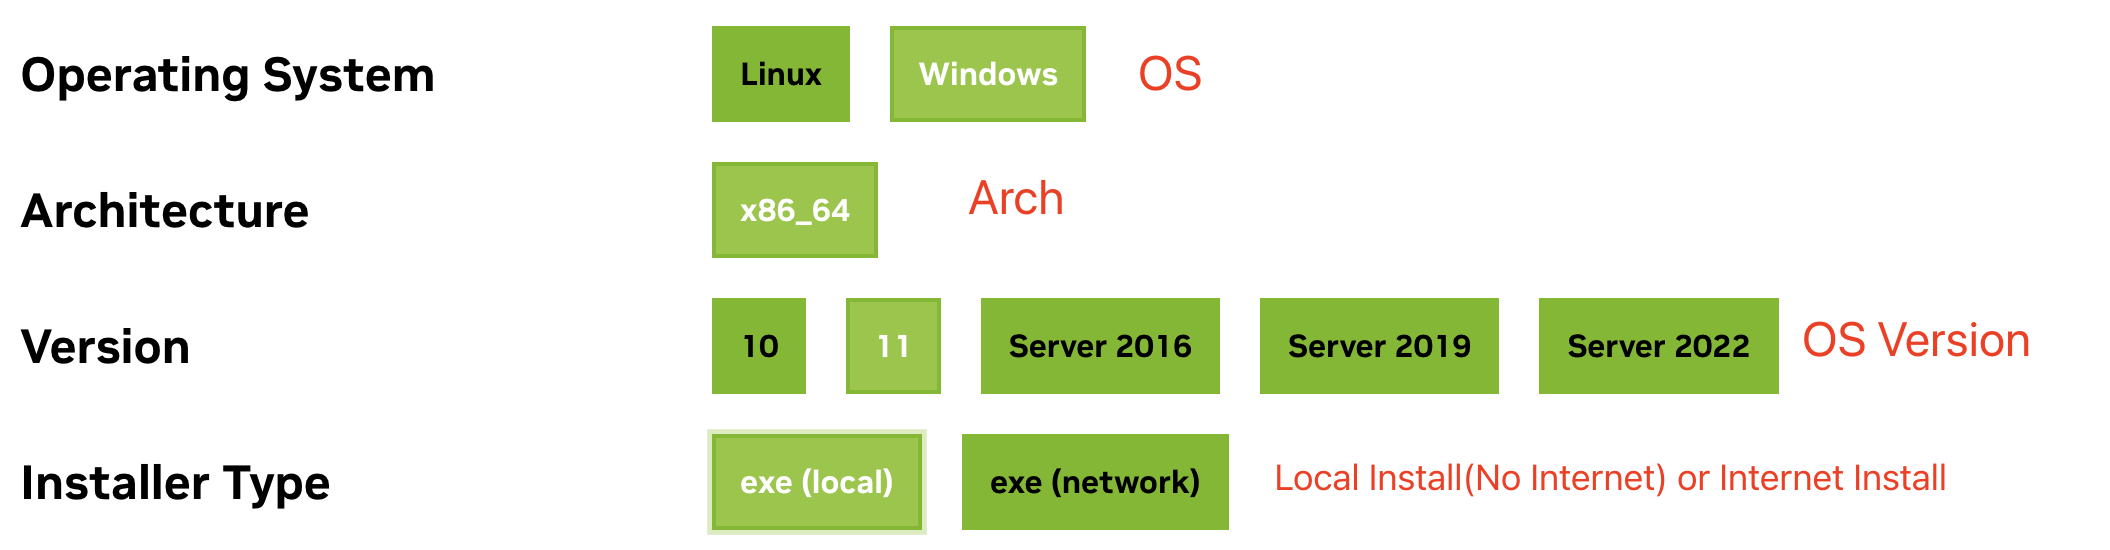
\includegraphics[width=0.8\textwidth]{cudadownload.png}
            \caption{CUDA Toolkit下载}
        \end{figure}
        \item 打开\url{https://anaconda.org/},搜索cudatoolkit,找到Pytorch/Tensorflow需要的
        cudatoolkit版本,然后进复制下载命令进行下载比如下面下载11.6版本的cudatoolkit。
        \begin{lstlisting}[style=bashstyle]
conda install deepmodeling::cudatoolkit
        \end{lstlisting}
    \end{enumerate}
    \item 运行刚刚下载可执行文件,全部默认安装即可,如果不在C盘安装会出现一些问题,有的程序会默认
    去C盘找CUDA的驱动文件导致无法运行。Linux不分盘所以无所谓。
    \item 安装完成后,需要配置环境变量,需要配置如下有名称的环境变量:
    \begin{lstlisting}[style=bashstyle]
CUDA_PATH = C:\Program Files\NVIDIA GPU Computing Toolkit\CUDA\v11.6
CUDA_PATH_V11_6 = C:\Program Files\NVIDIA GPU Computing Toolkit\CUDA\v11.6
    \end{lstlisting}
    和下面Path变量中的条目:
    \begin{lstlisting}[style=bashstyle]
C:\Program Files\NVIDIA GPU Computing Toolkit\CUDA\v11.6\bin
C:\Program Files\NVIDIA GPU Computing Toolkit\CUDA\v11.6\libnvvp
    \end{lstlisting}
    其中一个系统中可以有多个驱动版本,如果你想要使用什么版本,可以修改\texttt{CUDA\_PATH}
    以及将Path中的相应版本的路径上移到所有版本的路径之上即可实现快速的CUDA版本切换。
    \item 这时已经基本配置完成,\texttt{win+R}输入\texttt{powershell}打开powershell,
    输入下面的指令和看到下面输出的结果之后,说明CUDA已经安装成功。
    \begin{lstlisting}[style=bashstyle]
        (base) PS C:\Users\24692> nvcc -V
        nvcc: NVIDIA (R) Cuda compiler driver
        Copyright (c) 2005-2021 NVIDIA Corporation
        Built on Fri_Dec_17_18:28:54_Pacific_Standard_Time_2021
        Cuda compilation tools, release 11.6, V11.6.55
        Build cuda_11.6.r11.6/compiler.30794723_0
        (base) PS C:\Users\24692> nvidia-smi
        Mon Apr  8 09:38:47 2024
        +-----------------------------------------------------------------------------------------+
        | NVIDIA-SMI 551.86                 Driver Version: 551.86         CUDA Version: 12.4     |
        |-----------------------------------------+------------------------+----------------------+
        | GPU  Name                     TCC/WDDM  | Bus-Id          Disp.A | Volatile Uncorr. ECC |
        | Fan  Temp   Perf          Pwr:Usage/Cap |           Memory-Usage | GPU-Util  Compute M. |
        |                                         |                        |               MIG M. |
        |=========================================+========================+======================|
        |   0  NVIDIA GeForce RTX 3070 ...  WDDM  |   00000000:01:00.0 Off |                  N/A |
        | N/A   30C    P0             32W /  115W |       0MiB /   8192MiB |      0%      Default |
        |                                         |                        |                  N/A |
        +-----------------------------------------+------------------------+----------------------+
        
        +-----------------------------------------------------------------------------------------+
        | Processes:                                                                              |
        |  GPU   GI   CI        PID   Type   Process name                              GPU Memory |
        |        ID   ID                                                               Usage      |
        |=========================================================================================|
        |    0   N/A  N/A      2160    C+G   ...ekyb3d8bbwe\WsaClient\WsaClient.exe      N/A      |
        +-----------------------------------------------------------------------------------------+
    \end{lstlisting}
\end{enumerate}
\section{实验感想}

\newpage
\appendix
\section{源代码}
\end{document}